\section{Structure of Dominating Eigenvectors of the Full Hessian.}

% \znote{should we move thiis section to an earlier place?}
\label{sec:appendix_full_hessian}
Although it is not possible to apply Kronecker factorization to the full Hessian directly, we can construct an approximation of the top eigenvectors and eigenspace using similar ideas and our findings.In this section, we will always have superscript $(p)$ for all layer-wise matrices and vectors in order to distinguish them from the full versions.
As shown in \equationref{eqn:app_full_hessian} of \sectionref{sec:appendix_derivation}, we have the full Hessian of fully connected networks as 
\begin{equation}
    \HessL(\vtheta) = \E \left[\mF^\T_{\vx}\mA_\vx\mF_{\vx}\right] + \E\left[\sum_{i=1}^c \frac{\partial \ell(\vz,\vy)}{\evz_i} \nabla^2_\vtheta \evz_i \right],
\label{eqn:app_full_hessian_2}
\end{equation}
where
\begin{align}
    \mF^\T_\vx = \begin{pmatrix}
    \Gx^{(1)\T} \otimes \vx^{(1)}\\
    \Gx^{(1)\T}\\
    \Gx^{(2)\T} \otimes \vx^{(2)}\\
    \Gx^{(2)\T}\\
    \vdots\\
    \Gx^{(L)\T} \otimes \vx^{(n)}\\
    \Gx^{(L)\T}
    \end{pmatrix}.
\end{align}
In order to simplify the formula, we define \begin{equation}
    \tilde{\vx}^{(p)} = \begin{pmatrix}
    \vx^{(p)}\\
    1
    \end{pmatrix}
\end{equation} to be the extended input of the $p$-th layer. Thus, the terms in the Hessian attributed to the bias can be included in the Kronecker product with the extended input, and $\mF_\vx^\T$ can be simplified as
\begin{align}
\label{eqn:app_f_extened}
    \mF^\T_\vx = \begin{pmatrix}
    \Gx^{(1)\T} \otimes \tilde{\vx}^{(1)}\\
    \Gx^{(2)\T} \otimes \tilde{\vx}^{(2)}\\
    \vdots\\
    \Gx^{(L)\T} \otimes \tilde{\vx}^{(n)}\\
    \end{pmatrix}.
\end{align}

As discussed in several previous works \citep{sagun2016eigenvalues, papyan2018full, papyan2019measurements, fort2019emergent}, the full Hessian can be decomposed in to the G-term and the H-term. Specifically, the G-term is $\E \left[\mF^\T_{\vx}\mA_\vx\mF_{\vx}\right]$, and the H-term is $\E\left[\sum_{i=1}^c \frac{\partial \ell(\vz,\vy)}{\evz_i} \nabla^2_\vtheta \evz_i \right]$ in \equationref{eqn:app_full_hessian_2}.

Empirically, the G-term usually dominates the H-term, and the top eigenvalues and eigenspace of the Hessian are mainly attributed to the G-term. Since we focus on the top eigenspace, we can approximate our full Hessian using the G-term, as
\begin{equation}
     \HessL(\vtheta) \approx  \E\left[\mF^\T_{\vx}\mA_\vx\mF_{\vx}\right].
\end{equation}

In our approximation of the layer-wise Hessian $\HessL(\vw^{(p)})$ \equationref{eqn:decomp}, the two parts of the Kronecker factorization are the layer-wise output Hessian $\E[\mM^{(p)}_\vx]$ and the auto-correlation matrix of the input $\E[\vx^{(p)}\vx^{(p)\T}]$. Although we cannot apply Kronecker factorization to $\E\left[\mF^\T_{\vx}\mA_\vx\mF_{\vx}\right]$, we can still approximate its eigenspace using the eigenspace of the full output Hessian.

Note here that the full output Hessian is not a common definition. Let $\hat{m} = \sum_{p=1}^Lm^{(p)}$ be the sum of output dimension of each layer. We define a full output vector $\tilde{\vz}\in\R^{\hat{m}}$ by concatenating all the layerwise outputs together,
\begin{equation}
    \tilde{\vz} := \begin{pmatrix}
    \vz^{(1)}\\
    \vz^{(2)}\\
    \vdots\\
    \vz^{(L)}
    \end{pmatrix}.
\end{equation} 
We then define the full output Hessian is the Hessian w.r.t. $\tilde{\vz}$. Let the full output Hessian for a single input $\vx$ be $\mM_\vx\in\R^{\hat{m}\times \hat{m}}$. Similar to \equationref{eqn:app_layerwise_approx}, it can be expressed as
\begin{equation}
    \mM_\vx := \mH_\ell(\tilde{\vz}, \vx) = \mG_\vx^{\T}\mA_\vx\mG_\vx,
\end{equation}
where
\begin{equation}
    \mG^\T_\vx = \begin{pmatrix}
    \mG_\vx^{(1)\T}\\
    \mG_\vx^{(2)\T}\\
    \vdots\\
    \mG_\vx^{(L)\T}
    \end{pmatrix}
\end{equation}
similar to \equationref{eqn:app_f_extened}.
The full output Hessian for the entire training sample is thus
\begin{equation}
    \HessL(\tilde{\vz}) = \E[\mM_\vx] = \E[\mG_\vx^{\T}\mA_\vx\mG_\vx].
\end{equation}

We can then approximate the eigenvectors of the full Hessian $\HessL(\vtheta)$ using the eigenvectors of $\E[\mM_\vx]$. Let the $i$-th eigenvector of $\HessL(\vtheta)$ be $\vv_i$ and that of $\E[\mM_\vx]$ be $\vu_i$. We may then break up $\vu_i$ into segments corresponding to different layers as in
\begin{equation}
    \vu_i = \begin{pmatrix}
    \vu_i^{(1)}\\
    \vu_i^{(2)}\\
    \vdots\\
    \vu_i^{(L)}
    \end{pmatrix},
\end{equation}
where for all layer $p$, $\vu_i^{(p)}\in\R^{m^{(p)}}$.
Motivated by the relation between $\mG_\vx$ and $\mF_\vx$, the $i$-th eigenvector of $\HessL(\vtheta)$ can be approximated as the following. Let
\begin{equation}
    \vw_i = \begin{pmatrix}
    \vu_i^{(1)} \otimes \E[\tilde{\vx^{(1)}}]\\
    \vu_i^{(2)}\otimes \E[\tilde{\vx^{(2)}}]\\
    \vdots\\
    \vu_i^{(L)}\otimes \E[\tilde{\vx^{(L)}}]
    \end{pmatrix}.
\end{equation}
We then have
\begin{equation}
    \vv_i \approx \frac{\vw_i}{\|\vw_i\|}
\end{equation}
We can then use the Gram–Schmidt process to get the basis vectors of the approximated eigenspace.

Another reason for this approximation is that the expectation is the input of each layer $\E[\vx^{(p)}]$ dominates its covariance as shown in \sectionref{sec:appendix_xxT}. Thus, the approximate is accurate for top eigenvectors and also top eigenspace. For latter eigenvectors, the approximation would not be as accurate since this approximate loses all information in the covariance of the inputs.

We also approximated the eigenvalues using this approximation. Let the $i$-th eigenvalue of $\HessL(\vtheta)$ be $\lambda_i$ and that of $\E[\mM_\vx]$ be $\sigma_i$. We have
\begin{equation}
    \lambda_i \approx \sigma_i\|\vw_i\|^2.
\end{equation}

Below we show the approximation of the eigenvalues top eigenspace using this method. The eigenspace overlap is defined as in \definitionref{def:overlap}. We experimented on several fully connected networks, the results shown below are for F-$200^2$ (same as  \figureref{fig:eigeninfo_approx}(c)(d) in the main text), F-$200^4$, F-$600^4$, and F-$600^8$, all with dimension 50. The approximations are reasonably accurate.

\begin{figure}[H]
    \centering
    \begin{subfigure}[t]{0.5\textwidth}
        \centering
        \captionsetup{justification=centering}
        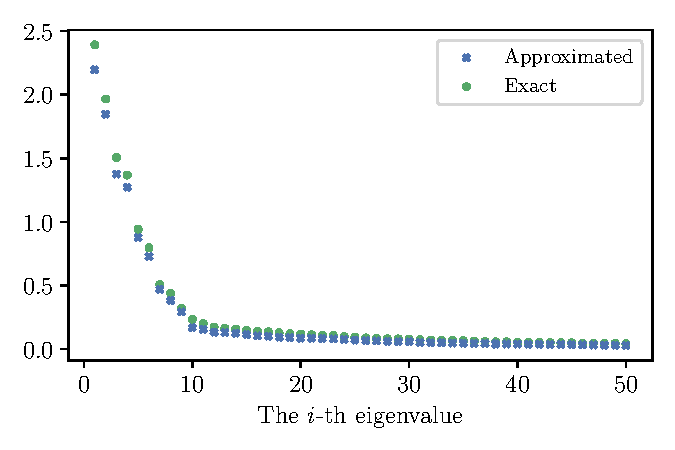
\includegraphics[width=\textwidth]{Appendix_Figures/Full_hessian/newplots/eigenval_fc2_200.pdf}
        \caption{Eigenvalues for F-$200^2$}
    \end{subfigure}%
    \begin{subfigure}[t]{0.5\textwidth}
        \centering
        \captionsetup{justification=centering}
        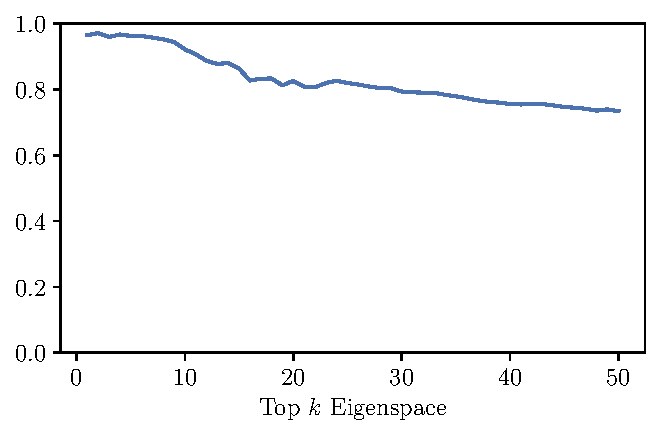
\includegraphics[width=\textwidth]{Appendix_Figures/Full_hessian/newplots/eigenvec_fc2_200.pdf}
        \caption{Eigenspace overlap for F-$200^2$}
    \end{subfigure}\\
    \begin{subfigure}[t]{0.5\textwidth}
        \centering
        \captionsetup{justification=centering}
        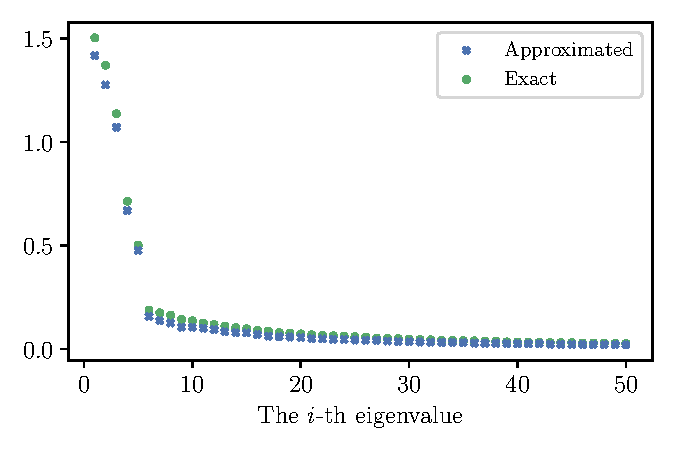
\includegraphics[width=\textwidth]{Appendix_Figures/Full_hessian/newplots/eigenval_fc4_200.pdf}
        \caption{Eigenvalues for F-$200^4$}
    \end{subfigure}%
    \begin{subfigure}[t]{0.5\textwidth}
        \centering
        \captionsetup{justification=centering}
        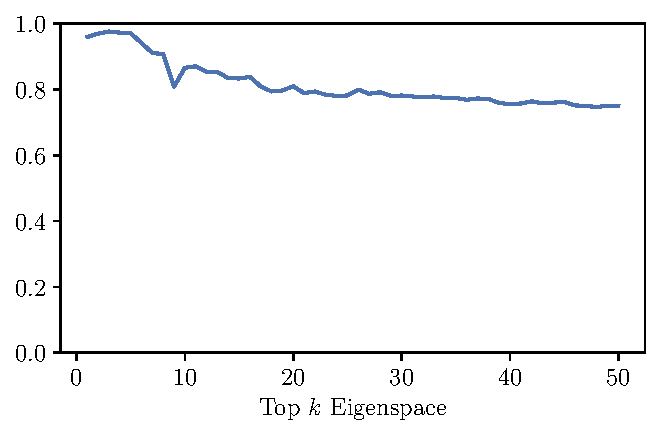
\includegraphics[width=\textwidth]{Appendix_Figures/Full_hessian/newplots/eigenvec_fc4_200.pdf}
        \caption{Eigenspace overlap for F-$200^4$}
    \end{subfigure}\\
    \begin{subfigure}[t]{0.5\textwidth}
        \centering
        \captionsetup{justification=centering}
        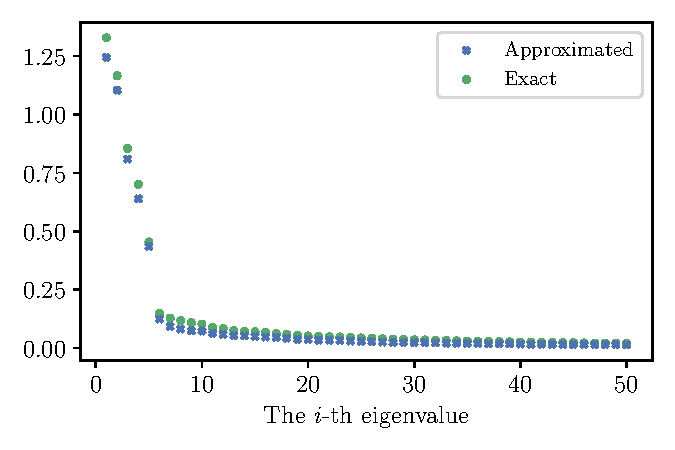
\includegraphics[width=\textwidth]{Appendix_Figures/Full_hessian/newplots/eigenval_fc4_600.pdf}
        \caption{Eigenvalues for F-$600^4$}
    \end{subfigure}%
    \begin{subfigure}[t]{0.5\textwidth}
        \centering
        \captionsetup{justification=centering}
        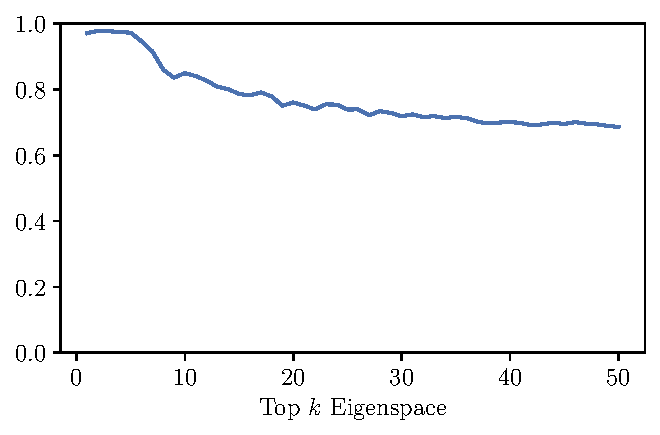
\includegraphics[width=\textwidth]{Appendix_Figures/Full_hessian/newplots/eigenvec_fc4_600.pdf}
        \caption{Eigenspace overlap for F-$600^4$}
    \end{subfigure}\\
    \begin{subfigure}[t]{0.5\textwidth}
        \centering
        \captionsetup{justification=centering}
        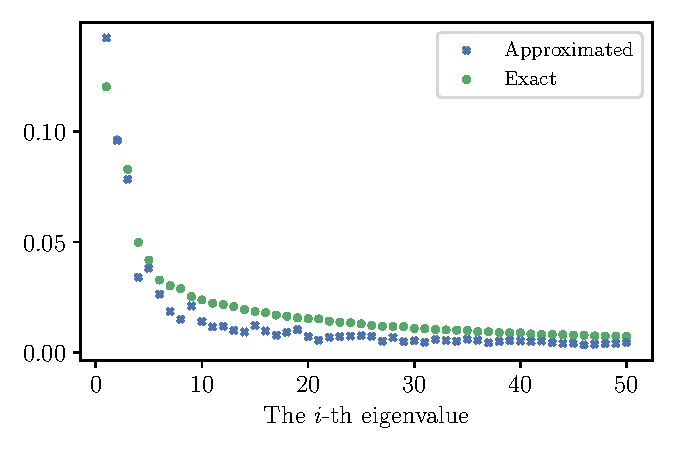
\includegraphics[width=\textwidth]{Appendix_Figures/Full_hessian/newplots/eigenval_fc8_600.pdf}
        \caption{Eigenvalues for F-$600^8$}
    \end{subfigure}%
    \begin{subfigure}[t]{0.5\textwidth}
        \centering
        \captionsetup{justification=centering}
        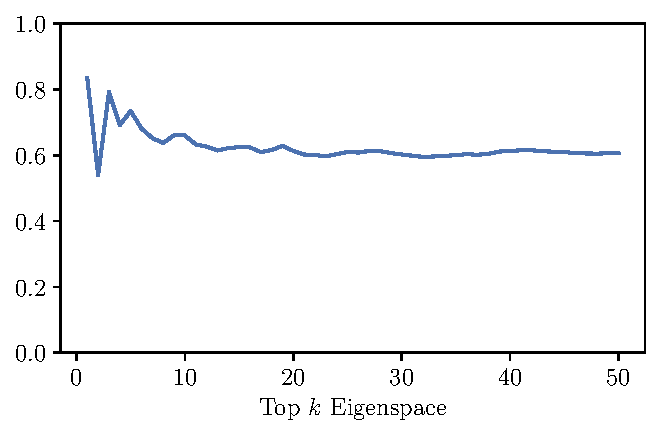
\includegraphics[width=\textwidth]{Appendix_Figures/Full_hessian/newplots/eigenvec_fc8_600.pdf}
        \caption{Eigenspace overlap for F-$600^8$}
    \end{subfigure}\\
    \caption{Top 50 Eigenvalues and Eigenspace approximation for full Hessian}
    \label{fig:Corrfc11}
\end{figure}
% \newpage
% \begin{figure}[h]
%     \centering
%     \vspace{-1em}
%     \subfigure[\small{Eigenvalues for F-$200^2$}]{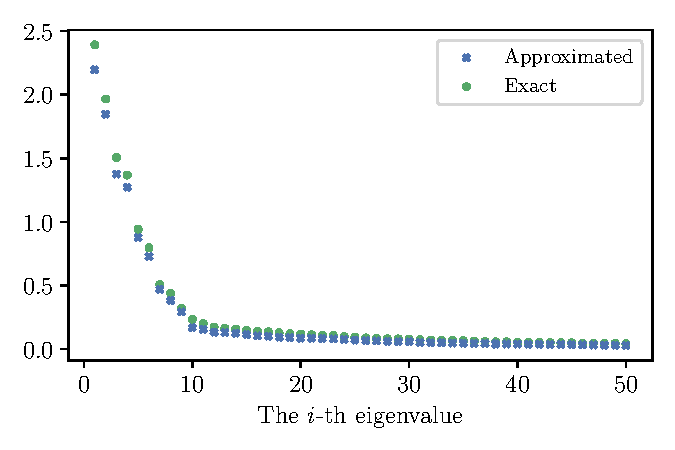
\includegraphics[width=0.42\linewidth]{Appendix_Figures/Full_hessian/newplots/eigenval_fc2_200.pdf}}
%     \subfigure[\small{Eigenspace overlap for F-$200^2$}]{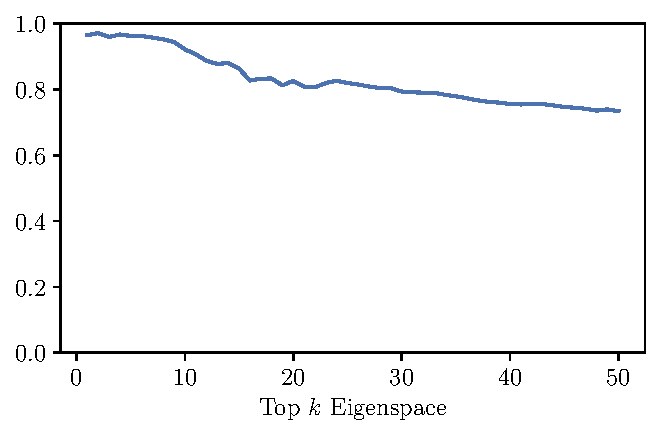
\includegraphics[width=0.42\linewidth]{Appendix_Figures/Full_hessian/newplots/eigenvec_fc2_200.pdf}}\\
%     \subfigure[\small{Eigenvalues for F-$200^4$}]{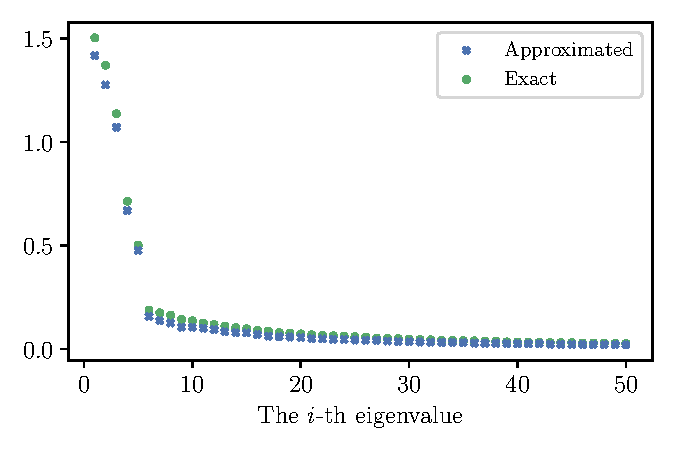
\includegraphics[width=0.42\linewidth]{Appendix_Figures/Full_hessian/newplots/eigenval_fc4_200.pdf}}
%     \subfigure[\small{Eigenspace overlap for F-$200^4$}]{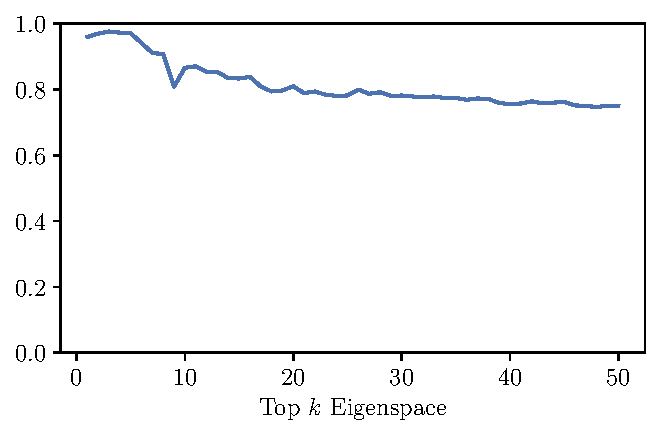
\includegraphics[width=0.42\linewidth]{Appendix_Figures/Full_hessian/newplots/eigenvec_fc4_200.pdf}}\\
%     \subfigure[\small{Eigenvalues for F-$600^4$}]{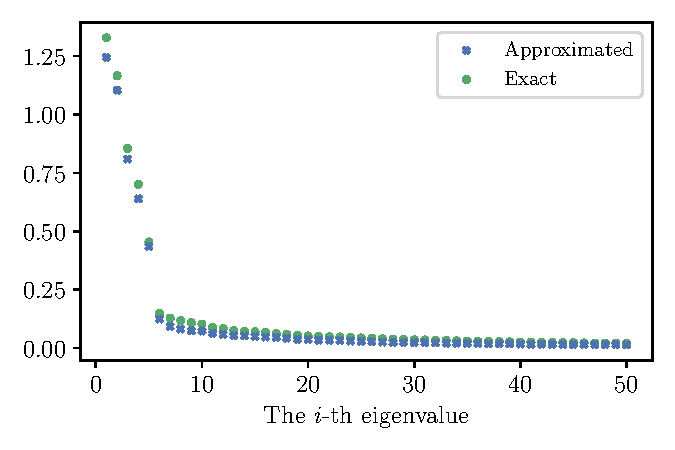
\includegraphics[width=0.42\linewidth]{Appendix_Figures/Full_hessian/newplots/eigenval_fc4_600.pdf}}
%     \subfigure[\small{Eigenspace overlap for F-$600^4$}]{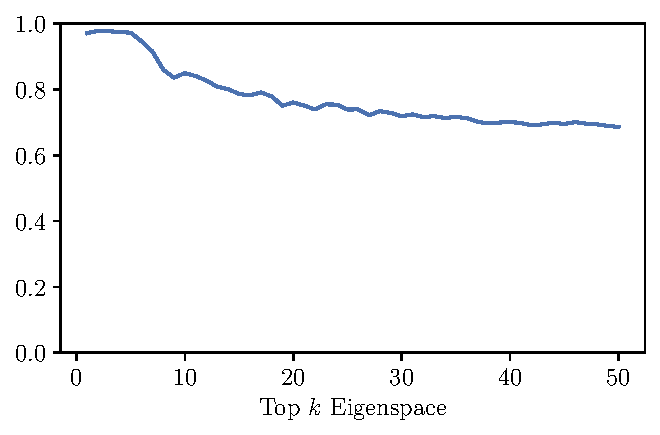
\includegraphics[width=0.42\linewidth]{Appendix_Figures/Full_hessian/newplots/eigenvec_fc4_600.pdf}}\\
%     \subfigure[\small{Eigenvalues for F-$600^8$}]{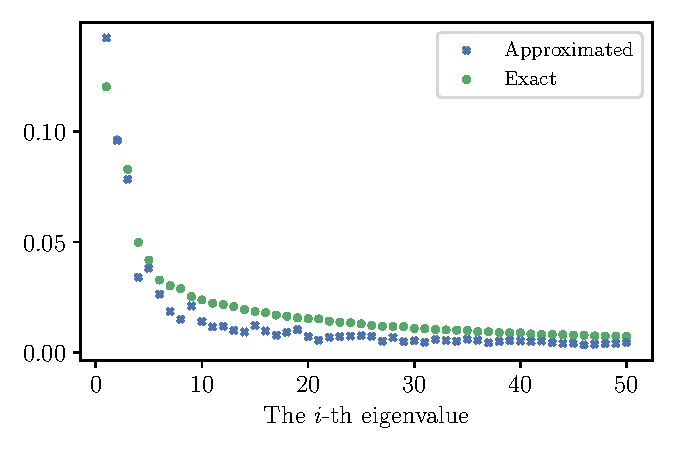
\includegraphics[width=0.42\linewidth]{Appendix_Figures/Full_hessian/newplots/eigenval_fc8_600.pdf}}
%     \subfigure[\small{Eigenspace overlap for F-$600^8$}]{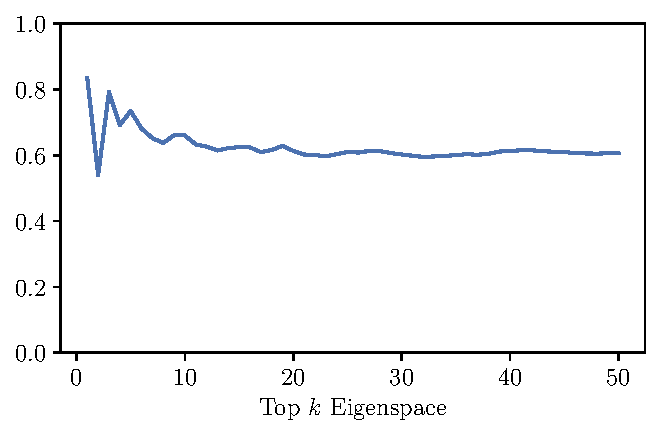
\includegraphics[width=0.42\linewidth]{Appendix_Figures/Full_hessian/newplots/eigenvec_fc8_600.pdf}}\\
%     \caption{Top 50 Eigenvalues and Eigenspace approximation for full Hessian}
%     \label{fig:Corrfc11}
%     \vspace{-1em}
% \end{figure}
\newpage